
%(BEGIN_QUESTION)
% Copyright 2006, Tony R. Kuphaldt, released under the Creative Commons Attribution License (v 1.0)
% This means you may do almost anything with this work of mine, so long as you give me proper credit

Anta at en elektrisk stekeovn er utstyrt med en temperaturfølsom styrebryter, som er koblet til et styrerelé for å sende elektrisk effekt til varmeelementet:

$$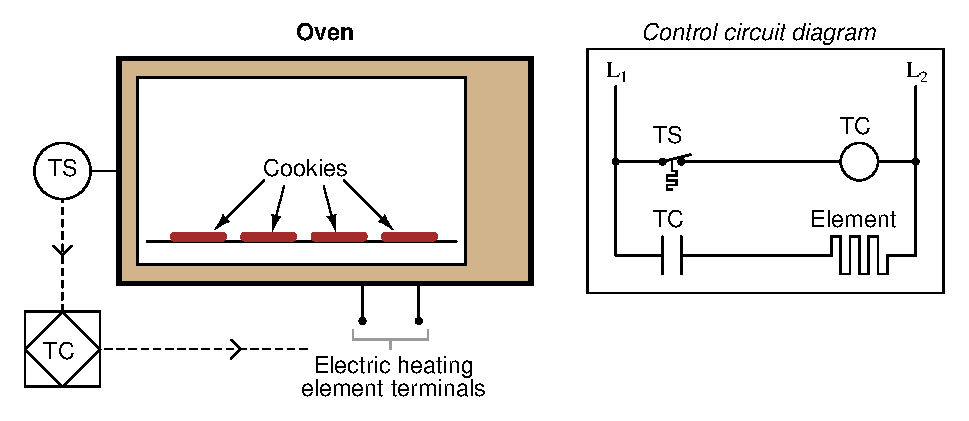
\includegraphics[width=15.5cm]{i01449x01.eps}$$

Hvordan vil dette enkle {\it av/på}-reguleringssystemet reagere på endringer i ovnstemperaturen, i forsøket på å holde temperaturen ved settpunktet? Forklar oppførselen til temperaturbryteren og relékretsen i detalj. Tegn også en graf av ovnstemperaturen over tid:

$$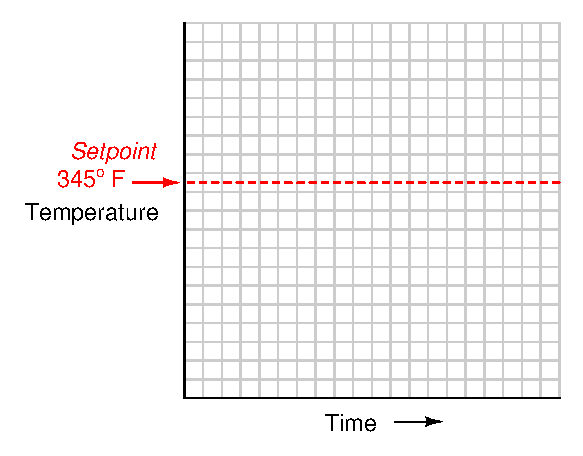
\includegraphics[width=15.5cm]{i01449x02.eps}$$

\underbar{file i01449}
%(END_QUESTION)





%(BEGIN_ANSWER)

Et enkelt {\it av/på}-reguleringssystem vil gi full effekt til varmeelementet hvis temperaturen er lavere enn settpunktet, og vil slå helt av effekten til varmeelementet hvis temperaturen er høyere enn settpunktet. Resultatet er en temperaturkurve som oscillerer rundt settpunktverdien over tid.
 
$$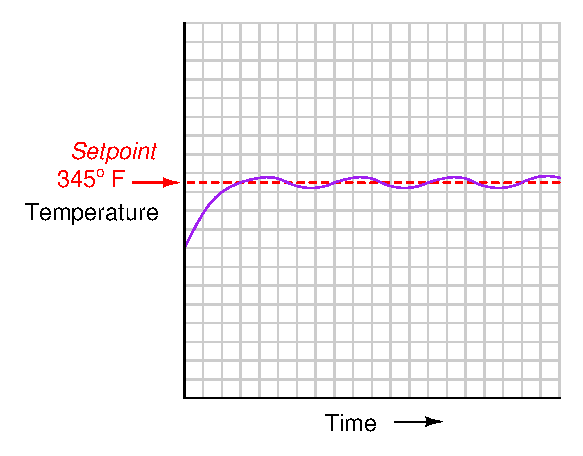
\includegraphics[width=15.5cm]{i01449x03.eps}$$

Som du ser, kan temperaturen aldri stabilisere seg på én enkelt verdi, fordi reguleringshandlingen er alt-eller-ingenting, og endres ut fra en enkel ``større enn''- eller ``mindre enn''-relasjon mellom prosessverdien og settpunktet.

Dette er et eksempel på et {\it lukket-sløyfe}-reguleringssystem. Regulerings-``sløyfen'' kan representeres i stigeplanskjemaet ved hjelp av årsakspiler:

$$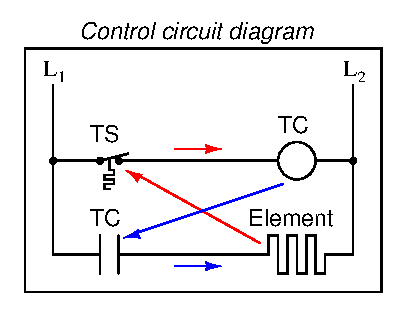
\includegraphics[width=15.5cm]{i01449x04.eps}$$


%(END_ANSWER)





%(BEGIN_NOTES)

\vskip 20pt \vbox{\hrule \hbox{\strut \vrule{} {\bf Virtuell feilsøking} \vrule} \hrule}

Dette spørsmålet egner seg godt som en ``Virtuell feilsøking''-øvelse. Når du presenterer diagrammet for studentene, forestiller du deg først en bestemt feil i systemet. Deretter presenterer du ett eller flere symptomer på denne feilen (noe en operatør eller annen bruker kan observere). Studentene foreslår så ulike diagnostiske tester for å identifisere feilens natur og plassering, slik teknikere ville gjort i praktisk feilsøking. Din oppgave er å fortelle hva resultatet ville blitt for hver foreslått test, og dokumentere resultatene slik at alle studentene kan se dem.

Under og etter øvelsen er det nyttig å stille oppfølgingsspørsmål som:

\begin{itemize}
\item{} Hva forteller resultatet av den siste diagnostiske testen deg om feilen?
\item{} Anta at resultatene av den siste diagnostiske testen var annerledes. Hva ville det resultatet fortalt deg om feilen?
\item{} Er den siste diagnostiske testen den beste vi kunne gjort?
\item{} Hva ville vært ideell testrekkefølge for å diagnostisere problemet i færrest mulig trinn?
\end{itemize}

%INDEX% Control, basics: on/off control
%INDEX% Process: cookie baking oven

%(END_NOTES)

